The Analog components layer contains 6 components. Five of the components will be actively interacting with each other. Being the pumps and heating elements will be controlled by the relays will be drawing power from the power supply. The thermometer will be interacting with the Digital component and Brew System Vessel Layers.

\begin{figure}[h!]
	\centering
	\graphicspath{.\images}
	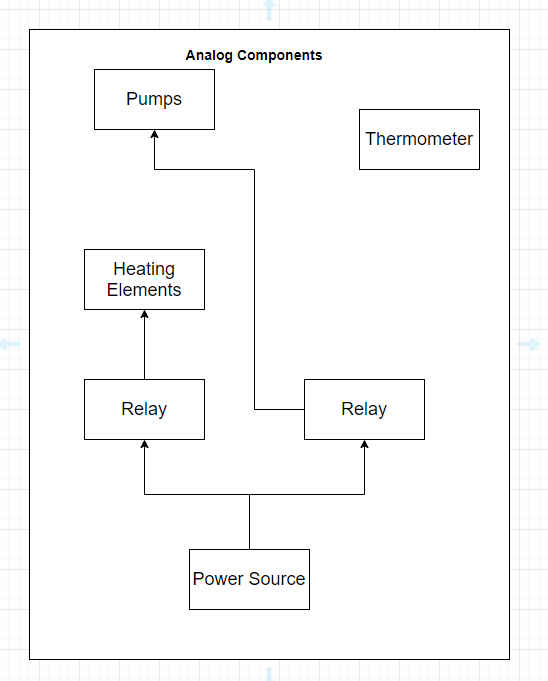
\includegraphics[scale=0.5]{images/analog_layer.PNG}
	\caption{Analog Components Layer}
\end{figure}

\subsection{Heating Elements Subsystem 1}
This subsystem is the temperature control subsystem used for managing temperature of the Hot Liquor tank and the Boiling Kettle. The Heating Elements will be managed by a relay that will be receiving control signals from a ESP32. 


\subsubsection{Assumptions}
We will be able to effectively manage the temperature of the Brewing system by increasing or decreasing temperature of heating elements. That is, logic on the digital components will be handling the optimal path to reach a certain temperature and the Relay will simply manage power to Heating Elements.  

\subsubsection{Responsibilities}
The subsystem will be responsible for temperature control of the brewing process.

\subsubsection{Subsystem Interfaces}

\begin {table}[H]
\caption {Subsystem interfaces} 
\begin{center}
    \begin{tabular}{ | p{4cm} | p{6cm} | p{5cm} | p{8cm} |}
    \hline
    Description & Inputs & Outputs \\ \hline
    Heating Elements & \pbox{5cm}{Power regulated by Relay} & \pbox{8cm}{Heat applied to Brew System}  \\ \hline
    Relay & \pbox{5cm}{Control information from ESP32} & \pbox{8cm}{Power to Heating Elements}  \\ \hline
    \end{tabular}
\end{center}
\end{table}


\subsection{Pump Control System Elements Subsystem 2}
This system will perform flow control from the Boiling Kettle to the Hot Liquor Tank. Like the Heating Elements, the Pumps will be controlled by a relay that is receiving control signals from an ESP32.    

\subsubsection{Assumptions}
The system will be designed to achieve a desired brew. You will only need this system to know when to turn on and off the pump from the Boiling Kettle to the Hot Liquor Tank.    

\subsubsection{Responsibilities}
The subsystem will be used for managing the pumping of liquid from the Boiling Kettle to the Hot Liquor Tank.

\subsubsection{Subsystem Interfaces}

\begin {table}[H]
\caption {Subsystem interfaces} 
\begin{center}
    \begin{tabular}{ | p{4cm} | p{6cm} | p{5cm} | p{8cm} |}
    \hline
    Description & Inputs & Outputs \\ \hline
    Heating Elements & \pbox{5cm}{Fluid from the Boiling Kettel \\ Power regulated by Relay} & \pbox{8cm}{Fluid to the Hot Liquor Tank}  \\ \hline
    Relay & \pbox{5cm}{Control information from ESP32} & \pbox{8cm}{Power moderation for Pumps}  \\ \hline
    \end{tabular}
\end{center}
\end{table}

\subsection{Power Relay Subsystem 3}
The power relay subsystem consist of the Relays and the Power Source. Relays will be used for managing power based on control signals from ESP32 to the Relays.     



\subsubsection{Assumptions}
The Relays will be connected to the Power Source and to the device it is controlling. The Relays will be able to operate on ESP32 inputs simply managing power to the devices.     

\subsubsection{Responsibilities}
This subsystem will be managing the power to devices that control elements of the Brew System Vessel.

\subsubsection{Subsystem Interfaces}

\begin {table}[H]
\caption {Subsystem interfaces} 
\begin{center}
    \begin{tabular}{ | p{5cm} | p{6cm} | p{5cm} | p{8cm} |}
    \hline
    Description & Inputs & Outputs \\ \hline
    Heating Elements & \pbox{5cm}{ESP32 control signals \\ Power from Power Source} & \pbox{5cm}{Power to device}  \\ \hline
    Relay & \pbox{5cm}{ESP32 control signals \\ Power from Power Source} & \pbox{5cm}{Power to device}  \\ \hline
    \end{tabular}
\end{center}
\end{table}


\subsection{Thermometer Subsystem 4}
This subsystem contains only one component, the Thermometer. It will be used for measuring the temperature of the Brew System and will relay that information to an ESP32.    



\subsubsection{Assumptions}
The Thermometer will have some other power supply. The ESP32 will take the temperature information and will know what to do when given the information.   

\subsubsection{Responsibilities}
This subsystem will be transporting temperature data from the Brew System to the necessary ESP32 were the information is required.  

\subsubsection{Subsystem Interfaces}

\begin {table}[H]
\caption {Subsystem interfaces} 
\begin{center}
    \begin{tabular}{ | p{5cm} | p{6cm} | p{5cm} | p{8cm} |}
    \hline
    Description & Inputs & Outputs \\ \hline
    Thermometer & \pbox{5cm}{Temperature measurements of Brew System Components} & \pbox{5cm}{Temperature data of Brew System}  \\ \hline
    
    \end{tabular}
\end{center}
\end{table}


